\startchapter{Framework}
\label{chapter:framework}

\section{Introduction}
Copilot works best in creating boilerplate and repetitive code patterns~\cite{Copilot-web}.
However, the code suggested by \cct{} like Copilot are found to have simple coding mistakes and security vulnerabilities. Several classes of errors have been discovered, which follow from the presence of these same errors in training data of Copilot~(shown in section~\ref{challenges}).
In Chapter~\ref{chapter:methodology}, we identified that Copilot does not perform well in detecting and suggesting Pythonic idioms and best practices in JavaScript.
The scope of capability and the quality of code suggestions made by \cct{} like Copilot is uncertain. 

In this chapter, we try to create a metric for answering \textbf{RQ-1} (What are the current boundaries of code completion tools) with a taxonomy of six software abstraction levels to help access the current capabilities of \cct{} such as Copilot. 
We explain each software abstraction level in the taxonomy and the capabilities required by \cct{} to satisfy the software abstraction level. 
We try to delineate where current \cct{} such as Copilot, are best able to perform and where more complex software engineering tasks overwhelm them using a software abstraction hierarchy where ``basic programming functionality'' such as code compilation and syntax checking is the lowest abstraction
level, while software architecture analysis and design are at the highest abstraction
level
Additionally, we use a sorting routine as an example scenario to show how a \cct{} code suggestion looks like in every level of abstraction in our taxonomy.

Finally, we try to address \textbf{RQ-2} (Given the current boundary, how far is it from suggesting design decisions?) with a discussion on the level of complexities and challenges involved in creating \cct{} that can satisfy design level compared to \cct{} satisfying code smells level in our taxonomy.

\subsection{Motivation}
To center our analysis on creating a software abstraction hierarchy to create a metric for answering \textbf{RQ-1} (What are the current boundaries of code completion tools), 
we leverage an analogous concept in the more developed (but still nascent) field of autonomous driving. 
Koopman has adapted the SAE Autonomous Driving safety levels~\cite{sae} to seven levels of autonomous vehicle safety hierarchy of needs shown in figure~\ref{fig:koopman_pyramid}. 

\begin{figure}[hbt!]
    \centering
    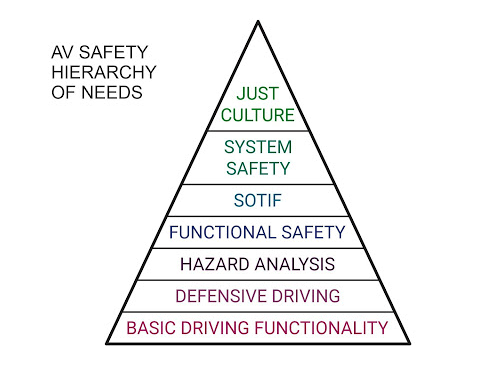
\includegraphics[width=\linewidth]{Figures/koopman_pyramid.png}
    \caption{Koopman's Autonomous Vehicle Safety Hierarchy of Needs~\cite{koopman}. SOTIF = safety of the intended function.}
    \label{fig:koopman_pyramid}
\end{figure}

The pyramid concept is derived from that of Maslow~\cite{Maslow1943}, such that addressing aspects on the top of the pyramid requires the satisfaction of aspects below. 
For example, before thinking about system safety (such as what to do in morally ambiguous scenarios), the vehicle must first be able to navigate its environment reliably (``Basic Driving Functionality'').

We think that a similar hierarchy exists in \AISE{}. Before worrying about software architecture issues, that is, satisfying system quality attributes such as performance and following idiomatic approaches, \AISE{} tools need to exhibit ``basic programming functionality''. This basic functionality is where most research effort is concentrated, such as program synthesis, \cct{}, and automated bug repair.

\section{Taxonomy}
\label{taxonomy}
Our taxonomy is a software abstraction hierarchy where ``basic programming functionality'' such as code compilation and syntax checking is the lowest abstraction level,
Software architecture analysis and design are at the highest abstraction level.
As we ascend the levels, just as with Koopman's pyramid in figure \ref{fig:koopman_pyramid}, 
software challenges rely more on human input and become more difficult to automate (e.g., crafting design rules vs. following syntax rules).

Figure~\ref{fig:taxonomy} shows the taxonomy of autonomy levels for \cct{}. The more abstract top levels depend on the resolution of the lower ones. As we move up the hierarchy, we require more human oversight of the AI; as we move down the hierarchy, rules for detecting problems are easier to formulate. Green levels are areas where \cct{} like Copilot works reasonably well, while red levels are challenging for Copilot based on tests shown in Chapter~\ref{chapter:methodology}.

\begin{figure}[hbt!]
    \centering
    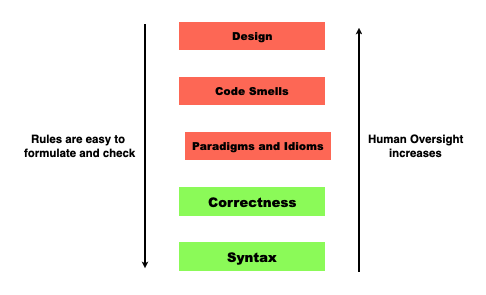
\includegraphics[width=\linewidth]{Figures/taxonomy.png}
    \caption{Hierarchy of software abstractions. Copilot cleared all green levels and struggled in red levels}
    \label{fig:taxonomy}
\end{figure}

Based on our tests with Copilot shown in chapter~\ref{chapter:methodology}, Copilot was able to generate syntactically correct code that solves the given programming task in the coding scenario~(shown in ~\repl{}).
This functionality covers the syntax and the correctness level in our software abstraction hierarchy.
As a result, Copilot stands at the correctness level of our taxonomy. 

The challenges further up the hierarchy are nonetheless more important for software quality attributes (QA)~\cite{Ernst2017} and for a well-engineered software system.
For example, an automated solution suggested by \cct{} to the top level of the taxonomy would be able to follow heuristics to engineer a well-designed software system, which would be easy to modify and scale to sudden changes in use.
\subsection{Syntax}
\label{syntax}
The syntax level is the lowest abstraction level in our taxonomy. This level includes the most basic programming functionality like syntax and code compilations. This level does not require the \cct{} suggested code to successfully perform the task but to suggest code without any obvious errors like syntax errors.

For example, consider a programming task of performing a sorting operation on a list of numbers. 
To satisfy this level of abstraction, \cct{} should suggest code that is syntactically correct without any compilation errors and the code is not required to perform the sorting operation correctly. 
Figure~\ref{fig:syntax} shows the sorting example and Python syntax suggestions from \cct{} at this abstraction level.

\begin{figure}[hbt!]
    \centering
    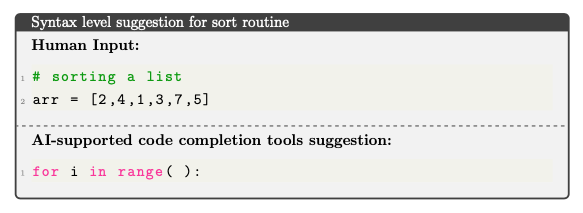
\includegraphics[width=\linewidth]{Figures/syntax.png}
    \caption{code suggestion of \cct{} at syntax level}
    \label{fig:syntax}
\end{figure}

The goal of this software abstraction level in our taxonomy is for a \cct{} to be able to suggest code without any syntactical errors.
The capabilities required by \cct{} to satisfy this level of abstraction are as follows:

\begin{enumerate}
    \item Suggested code should be syntactically correct.
    \item Suggested code should not produce any errors in code compilation.
\end{enumerate}

% \begin{tcolorbox}[title=Syntax level suggestion for sort routine,boxsep=.15mm]
%     %https://tex.stackexchange.com/questions/337909/tcolorbox-tcbline-style
% \textbf{Human Input:}
% \begin{lstlisting}[language={Python}]
% # sorting a list
% arr = [2,4,1,3,7,5]
% \end{lstlisting}
% \tcbline
% \textbf{\cct{} suggestion:}
% \begin{lstlisting}[language={Python}]
% for i in range( ):
% \end{lstlisting}
% \end{tcolorbox}
\subsection{Correctness}
\label{correctness}
Correctness is the second level of software abstraction in our taxonomy. 
\cct{} at this level should be capable of suggesting code that is not only syntactically correct but also solves the programming task. 
This level does not require \cct{} to suggest the best possible coding solution for the programming task but to be able to suggest a decent solution to the programming task which may or may not resolve all the edge cases of the given programming task.

For example, consider the programming task of performing a sorting operation on a list of numbers. To satisfy this level of abstraction, \cct{} should suggest a syntactically correct list sorting code, which is not required to be the most efficient way of sorting a list.
Figure~\ref{fig:correctness} shows the list sorting example and the Python code suggestion from \cct{} at this abstraction level, which performs the sorting operation.

\begin{figure}[hbt!]
    \centering
\begin{tcolorbox}[title=Correctness level suggestion for sort routine,boxsep=.15mm]
    %https://tex.stackexchange.com/questions/337909/tcolorbox-tcbline-style
\textbf{Human Input:}
\begin{lstlisting}[language={Python}]
# sorting a list
arr = [2,4,1,3,7,5]
\end{lstlisting}
\tcbline
\textbf{\cct{} suggestion:}
\begin{lstlisting}[language={Python}]
n = len(arr)
for i in range(n):
    for j in range(n-1):
        if arr[j] > arr[j+1]:
            temp = arr[j]
            arr[j] = arr[j+1]
            arr[j+1] = temp
print(arr)
\end{lstlisting}
\end{tcolorbox}
    \caption{Code suggestion of \cct{} at correctness level.}
    \label{fig:correctness}
\end{figure}

The goal of this software abstraction level in our taxonomy is for a \cct{} to be able to suggest a solution instead of the best one.
The capabilities required by \cct{} to satisfy this level of abstraction are as follows:

\begin{enumerate}
    \item Suggest a solution for a given programming task that may not be the optimal solution for that programming task.
    \item The solution suggested is not required to cover all the edge cases for that programming task.
    \item Satisfy requirements of all the levels below correctness in our taxonomy.
\end{enumerate}


\subsection{Paradigms and Idioms}
Paradigms and idioms are our taxonomy's third level of software abstraction. 
This level requires the code suggested by \cct{} to satisfy all the previous levels of abstractions and use common paradigms and language idioms in its code suggestions. 
These include common practices of solving a programming task. 

Returning to our running example of performing a sorting operation on a list of numbers. 
To satisfy this level of abstraction, \cct{} should suggest a syntactically correct list sorting code, using idiomatic ways in its code suggestions, like the Pythonic way of swapping items in a list~(line 5 in figure~\ref{fig:idioms}), As opposed to suggesting non-idiomatic approaches like creating another temporary variable to swap items in a list shown in correctness level~(figure~\ref{fig:correctness}).

Figure~\ref{fig:idioms} shows the sorting example and the Python code suggestions from \cct{} at this abstraction level.

\begin{figure}[hbt!]
    \centering
\begin{tcolorbox}[title=Idioms level suggestion for sort routine,boxsep=.15mm]
    %https://tex.stackexchange.com/questions/337909/tcolorbox-tcbline-style
\textbf{Human Input:}
\begin{lstlisting}[language={Python}]
# sorting a list
arr = [2,4,1,3,7,5]
\end{lstlisting}
\tcbline
\textbf{\cct{} suggestion:}
\begin{lstlisting}[language={Python}]
n = len(arr)
for i in range(n):
	for j in range(n-1):
		if arr[j] > arr[j+1]:
			arr[j], arr[j+1] = arr[j+1], arr[j]
print(arr)
\end{lstlisting}
\end{tcolorbox}
    \caption{Code suggestion of \cct{} at paradigms and idioms level.}
    \label{fig:idioms}
\end{figure}

The goal of this software abstraction level in the taxonomy is for \cct{} to detect and use commonly known idiomatic approaches and paradigms that occur in public code in its suggestions for suggesting code to solve a programming task.

The capabilities required by \cct{} to satisfy paradigms and idioms level of software abstraction are as follows:
\begin{enumerate}
    \item Identify common patterns like paradigms and language idioms in public code repositories~(training data).
    \item Use paradigms and language idioms in suggesting solutions for a programming task.
    \item Satisfy requirements of all the levels below paradigms and idioms in our taxonomy.
\end{enumerate}


\section{Design Smells}
Currently, Copilot does not support multi-file input, So it is not possible to evaluate its design suggestions, as software development process may include multiple folders with a file structure. 
Making Code completion tools adapt their suggestions to context specific issues such as variable naming conventions and formatting would be challenging as the existing guidelines are not standard in this space and mostly depend on context, The training dataset for AI driven development should also include rules such as idioms, best practices before tackling design level problems.
% Design smells or arch smells (Tushar Sharma)
\subsection{Design level}
Software design is the highest level of abstraction in our taxonomy. The goal of this level is to make \cct{} support the user in every software development process and suggest improvements.
To simplify the taxonomy of overall design processes in software development, we divided it into two subcategories: Module level design and System level design. 
\cct{} at the Module level design requires more user involvement in making design choices at the file level. Whereas, in system level design, \cct{} are more autonomous and require minimal input from the user in making design choices.

\subsubsection{Module level design}
\label{low_design}
Module level design is the first half of our taxonomy's design level of software abstraction.
This level requires the suggested code to be free of all known vulnerabilities and include test cases and continuous integration methods when applicable.
Code suggestions should also cover all the functional requirements of a given programming task.

\cct{} at this level should be able to pick and suggest the best applicable algorithm for a given coding scenario and be capable of following user-specified coding style guidelines.
For example, consider the task of sorting operation on a list of numbers. To satisfy this level of abstraction, \cct{} should suggest a syntactically correct list sorting code, using an algorithm that gives the best performance for that particular input scenario, like suggesting a quick sort algorithm~(avg time complexity = nlogn) instead of bubble sort algorithm~(avg time complexity = n\textsuperscript{2}).

The goal of this level in the taxonomy is for a \cct{} to be able to suggest appropriate design choices at the file level, considering the input from the user, like coding style guidelines, and help the user make design choices that satisfy all the functional requirements of the given programming task.

The capabilities required by a \cct{} to satisfy this level of abstraction are as follows
\begin{enumerate}
    \item Picking and suggesting the best applicable algorithm for a given scenario.
    \item Identify file level concerns in code files.
    \item Code suggestions should be free from all recognized vulnerabilities and warn the user if a vulnerability is found.
    \item Code suggestions should cover all the functional requirements of the given programming task.
    \item \cct{} should be able to suggest code with appropriate tests and Continuous Integration~(CI) when applicable.
    \item Code suggestions should follow user-specified coding style guidelines.
    \item Satisfy requirements of all previous levels of abstractions.
\end{enumerate}

% \begin{tcolorbox}[title=Code smells level suggestion for sort routine,boxsep=.15mm]
%     %https://tex.stackexchange.com/questions/337909/tcolorbox-tcbline-style
% \textbf{Human Input:}
% \begin{lstlisting}[language={Python}]
% # sorting a list
% arr = [2,4,1,3,7,5]
% \end{lstlisting}
% \tcbline
% \textbf{\cct{} suggestion:}
% \begin{lstlisting}[language={Python}, morekeywords={False, True}]
% swapped = False
% for i in range(len(arr)-1, 0, -1):
% 	for j in range(n):
% 		if arr[j] > arr[j+1]:
% 		    swapped = True
% 			arr[j], arr[j+1] = arr[j+1], arr[j]
% 	if not swapped:
% 	    break
% print(arr)
% \end{lstlisting}
% \end{tcolorbox}
\subsubsection{System level design}
\label{high_design}
System level design is the second half of the design level in our taxonomy. This level is the highest abstraction level with the highest human oversight and the most complex to define rules.
\cct{} at this level can suggest design decisions at the project level, like suggesting design patterns and architectural tactics with minimal input from the user.

This level requires the suggested code to suggest rational design practices in its code suggestions for a problem and satisfy all the previous levels of abstractions. Design practices depend on many factors like requirements and technical debt. \cct{} should be capable of considering all the relevant factors before suggesting a design practice and providing the reasoning for each choice to the user.

The main goal of this level in the taxonomy is for a \cct{} to help the user in every part of the software development process with minimal input from the user.

The capabilities required by a \cct{} to satisfy this level of abstraction are as follows
\begin{enumerate}
    \item Identify system level concerns in code files.
    \item Suggest design patterns and architectural tactics when prompted.
    \item Code suggestions should cover all the project's non-functional requirements.
    \item \cct{} should be able to identify the coding style followed and adapt its code suggestions.
    \item \cct{} should be able to make design decisions based on requirements and inform the user about those decisions.
    \item Satisfy requirements of all previous levels of abstractions.
\end{enumerate}

To make a \cct{} suggest design decisions is a very challenging task. 
Software design is very subjective, and software design concerns are still challenging to comprehend. 
This is because software design is one of the least concrete parts of the software development lifecycle, especially compared to testing, implementation, and deployment~\cite{sedesign}. 
Software design is typically carried out heuristically by drawing on the design team's knowledge, the project context (such as architecturally significant needs), and a constantly evolving set of patterns and styles from the literature. We discuss more on these challenges in Chapter~\ref{chapter:discussion}.
\section{AI-supported Software Development}
\label{cs2design}
We began this thesis by analyzing Copilot code suggestions on Pythonic idioms and best practices in Javascript to understand the current boundaries of \cct{} like Copilot using a software abstraction taxonomy.
In this section, we try to address \textbf{RQ-2} (Given the current boundary, how far is it from suggesting design decisions?) with a discussion on the complex nature of design decisions involving factors ranging from requirement analysis to maintenance, making it difficult for \cct{} like Copilot to detect the information from code files and suggest design decisions to satisfy the top software abstraction level of our taxonomy.
Additionally, we discuss our vision for \cct{} like Copilot to satisfy the design level in our taxonomy and outline the difficulty its underlying Codex LLM approach might run into.
Finally, we discuss how design choices change over time and outline the difficulties of \cct{} like Copilot to keep updating its suggestions and reflect the current design practices~(section~\ref{evolution}).

Software development is a challenging, complex activity: It is common for tasks to be unique and to call for the analysis of ideas from other domains. Solutions must be inventively modified to address the requirements of many stakeholders.
Software design is a crucial component of the software development activity since it determines the various aspects of the system, such as its performance, maintainability, robustness, security, etc.
Design is typically viewed in the context of software engineering as both a process~\cite{design} that a development team engages in and the specifications~\cite{designdef} that the team produces. 
Software design is typically carried out heuristically by pulling from the project context (such as architecturally significant needs), the design team's knowledge, and a constantly evolving set of patterns and styles from the literature. 

Automating this software design process, which is the most abstract element in the software development lifecycle, will be challenging. 
First, sufficient software design knowledge has to be collected to use as training data to create a good \cct{} that can suggest relevant architectural patterns. 
Software design generally occurs in various developer communication channels such as issues, pull requests, code reviews, mailing lists, and chat messages for multiple purposes such as identifying latent design decisions, design challenges, design quality, etc. 
Gathering all this data and generalizing those design decisions in training data to suggest relevant design choices to a user would be the vision for \cct{} to satisfy the design level.

Stack Overflow\footnote{\url{https://stackoverflow.com/}}, the most popular question and answer (Q\&A) forum used by developers for their software development queries~\cite{sotorrent}.
Software developers of all levels of experience conduct debates and deliberations in the form of questions, answers, and comments on Stack Overflow's extensive collection of topics about software development.
Due to these qualities, Stack Overflow is a top choice for software developers looking to crowdsource design discussions and judgments, making it a good source of training data for \cct{} for design choices.

Additionally, \cct{} at the design level should be capable of capturing design and module level concerns. 
These include capturing design patterns~(such as Observer) and architectural tactics~(such as Heartbeat) to improve and personalize suggestions.
The general understanding of a system's design that a software developer has is frequently susceptible to ``evaporation," which causes the developers to gradually lose knowledge of the design over time~\cite{martinse} making the process of gathering design data to train \cct{} a significant challenge.

Organizing software design information is an active research area. Previously, this design knowledge was organized largely manually because the information was heavily context-specific and a lack of large datasets. A study by Gorton et al.~\cite{databases} showed a semi-automatic approach to populate design knowledge from internet sources for a particular (big data) domain, which can be a helpful approach for collecting software design relevant data to train \cct{}.

Over the natural evolution of a software system, small changes accumulate, which can happen for various reasons, such as refactoring~\cite{fabio}, bug fixes~\cite{cotroneo}, implementation of new features, etc.
These changes can be unique. However, they frequently repeat themselves and follow patterns~\cite{changes}. 
Such patterns can provide a wealth of data for studying the history of modifications and their effects~\cite{martinchanges}, modification histories of fault fixes~\cite{daniel}, or the connections between code change patterns and adaptive maintenance~\cite{ijece}.
However, to use this data, \cct{} should be able to identify these complex patterns existing in public code~(training data). Current \cct{} like Copilot struggled to detect much simpler patterns like Pythonic idioms. There is no evidence currently to suggest they can identify even more complex design patterns.

Additionally, current \cct{} like Copilot does not support multi-file input. It is not possible to evaluate its current performance in design suggestions, as the software development process may include multiple folders with a file structure. 
For example, MVC pattern generally includes multiple files acting as Model, View, and Controller. Using the current limitations of input on Copilot, i.e., a code block or a code file, it is not possible for \cct{} to deduce that the project is using the MVC pattern and adapt its suggestion to follow the MVC pattern and not suggest code where Model communicated directly with View. \cct{} must be capable of making suggestions in multiple program units to accommodate these more abstract design patterns.

\cct{} should be able to adapt their suggestions to context-specific issues such as variable naming conventions and formatting. 
This would be challenging as the existing guidelines are not standard in this space and mostly depend on context.

\subsection{Evolution of design over time}
\label{evolution}
Software design is an ever-changing field that evolves along with technology, languages, and frameworks. As a result, either new design patterns are developed, or some existing ones are depreciated.
\cct{} need to update their code suggestions regularly to reflect the changes in design practices. 
This requires regularly updating the training data, and training costs are expensive.

Design patterns are solutions to recurring design issues that aim to improve reuse, code quality, and maintainability.
Design patterns have benefits such as decoupling a request from particular operations~(Chain of Responsibility and Command), making a system independent from software and hardware platforms~(Abstract Factory and Bridge), and independent from algorithmic solutions~(Iterator, Strategy, Visitor), or preventing implementation modifications~(Adapter, Decorator, Visitor). These design patterns are integral to software design and are used regularly in software development.
However, these design patterns evolve. For instance, with React Framework's introduction, many new design patterns were introduced, such as Redux and Flux, which were considered to be an evolution over the pre-existing MVC design pattern.
\cct{} trained before this evolution will not have any data of the new design patterns such as Redux and Flux, making them incapable of suggesting those design patterns to the user. 

Similarly, coding practices evolve. 
For example, in JavaScript, callbacks were considered the best practice in the past to achieve concurrency, which was replaced by promises. 
When the user has a goal to achieve asynchronous code, there are two ways to create async code: callbacks and promises. Callback allows us to provide a callback to a function, which is called after completion. With promises, you can attach callbacks to the returned promise object.
One common issue with using the callback approach is that when we have to perform multiple asynchronous operations at a time, we can easily end up with something known as callback hell.
As the name suggests, it is harder to read, manage, and debug. The simplest way to handle asynchronous operations is through promises. In comparison to callbacks, they can easily manage many asynchronous activities and offer better error handling.
This makes \cct{} be updated regularly to reflect new changes in coding practices and design processes of software development. 

Additionally, Bad Practices in using promises for asynchronous JavaScript like not returning promises after creation and forgetting to terminate chains without a catch statement, which are explained in documentation\footnote{\label{docs}\url{https://developer.mozilla.org/en-US/docs/Web/JavaScript/Guide/Using_promises}} and StackOverflow\footnote{\url{https://stackoverflow.com/questions/30362733/handling-errors-in-promise-all/}} are not known to Copilot and suggested code with those common anti-patterns as they could have occurred more frequently in Copilot training data. 
While testing, Copilot suggested code specifically mentioned in the JavaScript documentation as a common bad practice and anti-pattern\footref{docs}.
However, this is beyond the scope of this study and will be part of future work.

In conclusion, Software design is an abstract field of software development, where humans struggle to make correct design decisions using all their previous experience and various sources of information to satisfy the requirements of a system. 
Creating \cct{} to automate the software design process requires gathering relevant training data and regular updates to the training data to reflect the new changes in the evolution of the software development process. Further, the current Copilot approach of token-level suggestions needs to be upgraded to move beyond tokens~(shown in \ref{tokens}) to facilitate multi-file input to help make \cct{} capable of satisfying the design level of our taxonomy.
\section{Chapter Summary}
In summary, we start this chapter by showing the methodology used in addressing \textbf{RQ-1.2} (How do \cct{} manage to suggest non-smelly code?). We first introduced the study setup with the input to Copilot and how it was restricted to deriving the best practice from the input and how the suggestions from Copilot were evaluated. We sampled best practices from AirBNB JavaScript coding style guide~\cite{airbnb_code}, and then compared it against Copilot suggestions. Based on results shown in Table~\ref{tab:all_bp}, Copilot struggles to suggest the best practices from widely used coding standards in its suggestions. 

In this chapter, we showed that Copilot struggles to detect and follow coding style guides  present in public repositories of GitHub and always suggest code that follows those coding style guides. The ideal behavior of \cct{} like Copilot in solving this problem is to detect the coding style guideline from existing code in the project and always suggest code that follows the guideline.

In the next chapter (chapter~\ref{chapter:framework}), we illustrate our taxonomy inspired from autonomous driving levels on the software abstraction hierarchy in \AISE{}, and delineate where \cct{} are currently best able to perform, and where more complex software engineering tasks overwhelm them.